% Алгоритм FBP.

Как было показано ранее, алгоритм обратного проецирования легко описать и реализовать, но он не является вполне точным с математической точки зрения, поскольку опускает якобиан $|\omega|$. В результате этого, как правило, восстановленное изображение получается размытым, значения, близкие к началу координат, завышены, а далекие от начала координат, наоборот, занижены. Причина этого в том, что после дискретизации с равномерной сеткой по $s$ и $\theta$ через пиксели, близкие к началу координат, проходит большее количество дискретных прямых.

Алгоритм \textbf{filtered backprojection} состоит в использовании вместо \eqref{backprojection} более правильной формулы, выведенной в \eqref{fbp_proof}:
\begin{equation}
\label{filtered_backprojection}
    \left[ \mathcal{B}_{f}(p_\theta(s)) \right](x, y) = \mathcal{F}^{-1}\left[ |\omega| \hat{p}_\theta(\omega) \right]\left( x\cos\theta + y\sin\theta \right) d\theta.
\end{equation}

С точки зрения реализации следует добавить в алгоритм обратного проецирования дополнительный шаг: для каждого угла $\theta_i$ заменить <<сырые>> значения синограммы $p_{\theta_i}(s)$ на $\mathcal{F}^{-1}\left[ |\omega| \hat{p}_{\theta_i}(\omega) \right](s)$. Множитель $|\omega|$ называется \textbf{Ramp filter}.

\begin{figure}[!h]
    \centering
    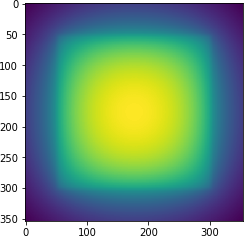
\includegraphics[width=0.3\linewidth]{backprojection_no_filter}
    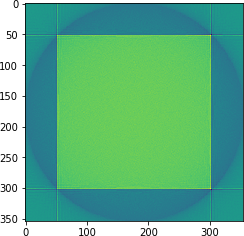
\includegraphics[width=0.3\linewidth]{backprojection_filtered}
    \caption{Восстановление белого квадрата из синограммы при помощи backprojection (слева) и filtered backprojection (справа).}
\end{figure}
